\chapter{密度泛函理论计算方法}\label{chap:dft}

本章讨论一种常用的求解固体电子结构的方法:\concept{密度泛函理论(DFT)}。
直接求解介质中的所有电子在库仑相互作用下的状态是极为困难的,但是我们将看到,原则上总是可以找到一个不依赖于具体系统的泛函,使得任何一个哈密顿量为\eqref{eq:electron-gas-hamiltonian}的系统的任何性质都可以通过最小化这个泛函得到。
这样的计算原则上不需要引入任何经验参数,因此称为\concept{第一性原理计算}。
虽然这么说,在实际的第一性原理计算中还是需要一些经验性的东西,如泛函的选取;并且,很多时候难以通过适当选取泛函来捕捉到一些特别近距离而强烈的相互作用(如Hubbard相互作用),从而需要使用所谓的DFT+$U$方法等。

\section{理论基础}

\subsection{Hohenberg-Kohn定理}

我们首先说明前述泛函的存在性。本节将通过两个定理,说明的确可以找到一个关于基态电子密度的泛函,使得我们只要最小化这个泛函即可原则上获得关于系统的所有性质。

我们有\concept{Hohenberg-Kohn第一定理}:基态非简并、动能项和相互作用势能项固定、外加势能项是只和位置有关的单粒子算符的哈密顿量\eqref{eq:electron-gas-hamiltonian-sq}的基态电子密度可以唯一确定哈密顿量,即基态电子密度和这类哈密顿量有一一对应的关系。(或者,说得更加明确一些,基态电子密度和\eqref{eq:electron-gas-hamiltonian}中的$V(\vb*{r})$是一一对应的)
其中,电子密度为
\begin{equation}
    \rho(\vb*{r}) = \mel{\Psi}{{\psi}^\dagger(\vb*{r}) {\psi}(\vb*{r})}{\Psi}.
\end{equation}
这个定理的证明如下。如果两个哈密顿量是相同的那么它们当然会给出一样的基态电子密度。
而如果两个哈密顿量不相同却给出了一样的基态电子密度,设这两个哈密顿量是
\[
    {H}_1 = {T} + {V}_\text{int} + {V}_1
\]
和
\[
    {H}_2 = {T} + {V}_\text{int} + {V}_2,
\]
且记每个粒子的外加势能分别是$V_1(\vb*{r})$和$V_2(\vb*{r})$,它们的基态分别是$\ket{\Psi_1}$和$\ket{\Psi_2}$,基态能量为$E_1$和$E_2$,则
\[
    \mel{\Psi_1}{{T} + {V}_1}{\Psi_1} = E_1, \quad \mel{\Psi_2}{{T} + {V}_2}{\Psi_2} = E_2,
\]
且由基态唯一性有
\[
    \mel{\Psi_2}{{T} + {V}_1}{\Psi_2} > E_1, \quad \mel{\Psi_1}{{T} + {V}_2}{\Psi_1} > E_2,
\]
两式相减就得到
\[
    \mel{\Psi_1}{{V}_2 - {V}_1}{\Psi_1} > E_2 - E_1, \quad \mel{\Psi_2}{{V}_1 - {V}_2}{\Psi_2} > E_1 - E_2,
\]
而
\[
    \mel{\Psi}{{V}}{\Psi} = \int \dd[3]{\vb*{r}} \mel{\Psi}{{\psi}^\dagger(\vb*{r}) V(\vb*{r}) {\Psi}(\vb*{r})}{\psi} = \int \dd[3]{\vb*{r}} = \int \dd[3]{\vb*{r}} \rho(\vb*{r}) V(\vb*{r}),
\]
于是上式等价于
\[
    \int \dd[3]{\vb*{r}} \rho_1(\vb*{r}) (V_2(\vb*{r}) - V_1(\vb*{r})) > E_2 - E_1, \quad \int \dd[3]{\vb*{r}} \rho_2(\vb*{r}) (V_1(\vb*{r}) - V_2(\vb*{r})) > E_1 - E_2.
\]
既然$\rho_1(\vb*{r}) = \rho_2(\vb*{r})$,以上两个不等式意味着$0 > 0$,而这当然是不正确的,因此如果基态电子密度一样,那么哈密顿量就不可能不同。
这就证明了Hohenberg-Kohn第一定理。

Hohenberg-Kohn第一定理意味着,只需要基态电子密度就足够确定一个\eqref{eq:electron-gas-hamiltonian-sq}型体系,因为\eqref{eq:electron-gas-hamiltonian}中的动能项都是一样的。
因此这样一个体系的所有性质都可以写成基态电子密度的泛函。
这个看起来不可思议的结论来自电子-原子核体系\eqref{eq:electron-gas-hamiltonian}只是所有可能的体系中的很小一部分这一事实。

实际上,还可以将Hohenberg-Kohn第一定理推广到可能具有简并基态的哈密顿量上。定义\concept{Levy-Lieb泛函}:
\begin{equation}
    \begin{aligned}
        E_\text{LL} [V_\text{ext}(\vb*{r}), \rho(\vb*{r})]  &= \underbrace{\min_{\rho[\psi]=\rho(\vb*{r})} \mel{\psi}{{T} + {V}_\text{int}}{\psi}}_{F_\text{LL}} + \int \dd[3]{\vb*{r}} \rho(\vb*{r}) V_\text{ext} (\vb*{r}) \\
        &= \min_{\rho[\psi]=\rho(\vb*{r})} \mel{\psi}{{T} + {V_\text{int}} + {V}_\text{ext}}{\psi},
    \end{aligned}
    \label{eq:levy-lieb}
\end{equation}
它的取值肯定不会低于系统的基态能量,而如果$\rho(\vb*{r})$正好是外加势$V_\text{ext}(\vb*{r})$对应的电子密度,那么$\ket{\psi}$的取值范围当中肯定包括所有基态,于是$E_\text{LL}$给出了基态能量,而且这是该泛函的极小值。
既然如此,记$\rho_0(\vb*{r})$为$V_\text{ext}(\vb*{r})$对应的电子密度,固定外加势不动对Levy-Lieb泛函做优化,其中$\rho(\vb*{r})$满足约束
\[
    \int \dd[3]{\vb*{r}} \rho(\vb*{r}) = 1,
\]
那么由拉格朗日乘子法,一定有%
\footnote{注意$\lambda$是一个常数而不是一个场,而变分通常都是一个场。}%
\[
    \eval{\fdv{E_\text{LL}}{\rho(\vb*{r})}}_{\rho(\vb*{r}) = \rho_0 (\vb*{r})} = \lambda,
\]
这也就是说
\[
    \eval{\fdv{F_\text{LL}}{\rho(\vb*{r})}}_{\rho(\vb*{r}) = \rho_0(\vb*{r})} + V_\text{ext} = \lambda,
\]
而可以通过别的优化方程计算出$\lambda$,这样实际上我们已经写出了$V_\text{ext}$关于$\rho_0(\vb*{r})$的表达式(可以差一个常数),因此可以从$\rho_0(\vb*{r})$把$V_\text{ext}$恢复出来,也即所有$V_\text{ext}$和所有可能的基态电子密度是一一对应的。
因此Hohenberg-Kohn第一定理对具有简并基态的\eqref{eq:electron-gas-hamiltonian-sq}型系统也使用。
总之,求解出了基态电子密度,我们就获得了一个系统的所有信息,关于这个系统的所有物理量都可以通过基态电子密度的某个泛函计算出来。

一旦有了以上结论,就得到\concept{Hohenberg-Kohn第二定理},也即,基态电子密度是固定了$V_\text{ext}$之后的Levy-Lieb泛函(此时称为\concept{能量泛函})的极小值,可以使用变分原理求出。
这个定理的证明只不过是把上面的论述倒过来使用而已:上面的论述表明给定$\rho_0(\vb*{r})$,通过泛函变分可以计算出$V_\text{ext}$,给定了$V_\text{ext}$通过泛函变分也可以计算出$\rho_0(\vb*{r})$,既然基态电子密度让能量泛函最小。
实际上,记外加势能为$V(\vb*{r})$的能量泛函为$E[\cdots]$,用于求解基态电子密度的变分问题就是
\begin{equation}
    \var \left( E[\rho(\vb*{r})] - \mu \left( \int \dd[3]{\vb*{r}} \rho(\vb*{r}) - N \right) \right) = 0.
    \label{eq:dft-variation-principle}
\end{equation}
这个$\mu$的形式看起来很眼熟,似乎就是化学势。实际上如果近独立电子近似成立,它真的就是零温化学势,即费米能。这一点我们在\autoref{sec:single-electron-in-dft}中可以看到。

\subsection{Kohn-Sham方法}

现在的问题是,给定一个$V_\text{ext}$,怎么写出$E[\rho]$?
为了让我们能够写下一个明确的能量泛函,需要引入一些辅助手段。
对一个给定的电子数密度$\rho(\vb*{r})$,构造一个乘积态
\begin{equation}
    \ket{\Psi} = \prod_{i=1}^N {\psi}^\dagger_i \ket{0},
    \label{eq:dft-state}
\end{equation}
使得这个乘积态对应的电子数密度就是$\rho(\vb*{r})$,且它正好是\eqref{eq:levy-lieb}中的让$F_\text{LL}$取最小值的那个$\ket{\Psi}$,或者至少与之非常接近。
如果我们最后需要计算的物理量和$\rho(\vb*{r})$之间的关系是足够平滑的,用拟设\eqref{eq:dft-state}就能够得到很好的结果。
需注意$\ket{\psi}$是乘积态并不意味着密度泛函理论是一个单粒子理论,密度泛函理论并不断言$\ket{\psi}$是系统实际的状态,它只是用来辅助计算的一个数学技巧而已。
这样,就有%
\begin{equation}
    E[\rho] = \mel{\Psi}{{H}}{\psi} = \mel{\psi}{{T} + {V}_\text{ext} + {V}_\text{int}}{\Psi}.
\end{equation}
记${\psi}_i^\dagger$产生的单粒子波函数为$\phi(\vb*{r})$,则
\begin{equation}
    \rho(\vb*{r}) = \sum_{i=1}^N \abs{\phi_i(\vb*{r})}^2,
    \label{eq:kohn-sham-density}
\end{equation}
或者,为了避免占据数突变造成计算上的困难,我们可以设
\begin{equation}
    \rho(\vb*{r}) = \sum_i f_i \abs{\phi_i(\vb*{r})}^2,
\end{equation}
其中$f_i$通常就是费米分布函数,总之是一个在费米面以下基本上处处为$1$而在费米面以上(在这里就是$i > N$)基本上处处为$0$的函数。
动能和外加势能都是单体算符,因此以$\ket{\Psi}$为本征态之一。动能项应为
\begin{equation}
    T_\text{s} = \mel{\Psi}{{T}}{\Psi} = - \frac{1}{2m} \sum_i \int \dd[3]{\vb*{r}} \phi_i^*(\vb*{r}) \laplacian \phi_i(\vb*{r}),
\end{equation}
这里下标s表示这个动能项实际上是假定$\ket{\Psi}$是自由理论中的多粒子态而计算出来的;如果$\ket{\Psi}$实际上具有强关联效应,那么用它计算动能就会不对头。
但是,$\ket{\Psi}$和系统实际的波函数也没有什么直接关系,$T_\text{s}$和真实的$\mel*{\Psi}{T}{\Psi}$有差别这件事不会有什么影响,因为反正它们的差最后会在$E_\text{XC}$中得到补偿。
单粒子外加势能项为
\begin{equation}
    V = \mel{\Psi}{{V}_\text{ext}}{\Psi} = \sum_i \int \dd[3]{\vb*{r}} V_{\text{ext}}(\vb*{r}) \phi_i^*(\vb*{r}) \phi_i(\vb*{r}) = \int \dd[3]{\vb*{r}} \rho(\vb*{r}) V_\text{ext}(\vb*{r}),
\end{equation}
而二体的库伦势却会带来很大麻烦。当然,如果采用托马斯-费米近似,即认为不同电子的电子云几乎没有交叠,则唯一剩下的一项就是
\[
    \mel{\Psi}{{V}_\text{int}}{\Psi} \approx V_H = \frac{1}{2} \int \dd[3]{\vb*{r}} \int \dd[3]{\vb*{r}'} \frac{e^2 \rho(\vb*{r}) \rho(\vb*{r}')}{\abs{\vb*{r} - \vb*{r}'}},
\]
但是正如我们在Hartree-Fock近似中看到的那样,在电子云存在交叠的情况下会有一个交换能,而且Hartree-Fock近似与真实能量还存在偏差(称为\concept{关联能},这种误差肯定会有因为Hartree-Fock近似是一个平均场理论)。既然$\mel{\psi}{{V}_\text{int}}{\psi}$和上式都是$\rho(\vb*{r})$的泛函,交换能也应该是$\rho(\vb*{r})$的泛函,但我们根本写不出它的解析表达式。
因此实际工作中必须猜测一个\concept{交换-关联能}$E_\text{XC}$,从而写出能量泛函
\begin{equation}
    \begin{aligned}
        E[\rho(\vb*{r})] &= T_\text{s}[\rho(\vb*{r})] + V[\rho(\vb*{r})] + V_H[\rho(\vb*{r})] + E_\text{XC} [\rho(\vb*{r})] \\
        &= - \frac{1}{2m} \sum_i \int \dd[3]{\vb*{r}} \phi_i^*(\vb*{r}) \laplacian \phi_i(\vb*{r})
        + \int \dd[3]{\vb*{r}} \rho(\vb*{r}) V_\text{ext}(\vb*{r}) \\
        &+ \frac{1}{2} \int \dd[3]{\vb*{r}} \int \dd[3]{\vb*{r}'} \frac{e^2 \rho(\vb*{r}) \rho(\vb*{r}')}{\abs{\vb*{r} - \vb*{r}'}} + E_\text{XC} [\rho(\vb*{r})].
    \end{aligned}
    \label{eq:kohn-sham-functional}
\end{equation}
将\eqref{eq:kohn-sham-functional}对$\phi_i^*(\vb*{r})$做优化,即求解
\begin{equation}
    \var \left( E[\rho(\vb*{r})] - \sum_i \epsilon_i \left( \int \dd[3]{\vb*{r}} \phi_i^*(\vb*{r}) \phi_i(\vb*{r}) - 1 \right) \right) = 0,
    \label{eq:dft-variation-principle-shem}
\end{equation}
得到
\begin{equation}
    \left( - \frac{1}{2 m} \laplacian + \int \dd[3]{\vb*{r}'} \frac{\rho(\vb*{r}')}{\abs{\vb*{r} - \vb*{r}'}} + V_\text{ext}(\vb*{r}) + V_\text{XC}(\vb*{r}) \right) \phi_i(\vb*{r}) = \epsilon_i \phi_i(\vb*{r}),
    \label{eq:kohn-sham-eq}
\end{equation}
其中
\begin{equation}
    V_\text{XC}(\vb*{r}) \phi_i(\vb*{r}) = \fdv{E_\text{XC}[\rho(\vb*{r})]}{\phi^*_i(\vb*{r})} = \fdv{E_\text{XC}[\rho(\vb*{r})]}{\rho(\vb*{r})} \phi_i(\vb*{r}).
\end{equation}
\eqref{eq:kohn-sham-eq}是一个有$N$个显含$\rho(\vb*{r})$的方程的方程组,称为\concept{Kohn-Sham方程}。
它们与\eqref{eq:kohn-sham-density}联立就给出了所有的$\psi_i(\vb*{r})$,并立即可以求出$\rho(\vb*{r})$,从而完全解出了系统的一切性质。
基本上数值求解\eqref{eq:kohn-sham-eq}的过程可以概括为\autoref{alg:basic-kohn-sham}。

\begin{algorithm}

    \DontPrintSemicolon
    \SetAlgoLined

    \KwData{初始电子密度$\rho_0(\vb*{r})$,容差$\epsilon$,交换关联泛函选取$E_\text{XC}[\rho(\vb*{r})]$}
    \KwResult{Kohn-Sham波函数$\phi_i(\vb*{r})$和对应的本征值$\epsilon_i$}
    
    $i = 1$ \;
    将$\rho_0(\vb*{r})$代入\eqref{eq:kohn-sham-eq}求解得到$\phi_n^{(1)}$和$\epsilon_n^{(1)}$ \;
    将$\phi_n^{(1)}$代入\eqref{eq:kohn-sham-density}计算得到$\rho_1(\vb*{r})$ \;
    \While{$\rho_i(\vb*{r})$和$\rho_{i-1}(\vb*{r})$的差别大于容差$\epsilon$}{
        将$\rho_i$代入\eqref{eq:kohn-sham-eq}求解得到$\phi_n^{(i+1)}$和$\epsilon_n^{(i+1)}$ \;
        $i = i + 1$ \;
    }
    
    \Return{波函数$\phi^{(i)}_n$和本征值$\epsilon^{(i)}_n$}\;

    \caption{Kohn-Sham方程的自洽求解}
    \label{alg:basic-kohn-sham}
\end{algorithm}

我们又一次看到,Kohn-Sham方程的形式基本上就是“一个电荷背景中的单电子”,只不过电子-电子库伦相互作用不仅包括平方反比律(实际上就是Hartree项),还包括一个(形式难以一般地写出的)$V_\text{XC}$,即我们需要求解有效势能
\begin{equation}
    V_\text{eff}(\vb*{r}) = V_\text{ext}(\vb*{r}) + V_\text{XC}(\vb*{r}) + \int \dd[3]{\vb*{r}'} \frac{\rho(\vb*{r}')}{\abs{\vb*{r} - \vb*{r}'}}
\end{equation}
如果近独立电子近似成立,$\epsilon_i$可能就是电子能级。我们将在\autoref{sec:single-electron-in-dft}中看到这一点。
需注意Kohn-Sham方程的解唯一确凿无疑的物理意义就是电荷密度;$\epsilon_i$和$\phi_i$有什么意义是不完全确定的。

\section{后处理和物理量测量}

本节讨论Kohn-Sham方程求解完成后怎样从计算结果解读出我们需要的各个物理量。

\subsection{和基态电子密度有解析形式关系的量}

基态能量实际上就是能量泛函作用在基态电子密度$\rho(\vb*{r})$之后的结果。

\subsection{单电子诠释和能带}\label{sec:single-electron-in-dft}

在待计算的系统确实适用单电子诠释时,我们将\eqref{eq:kohn-sham-eq}和\eqref{eq:dyson-wave-eq}对比,很容易看出两者的相似之处。
如果Hartree项加上$V_\text{XC}$构成对自能$\Sigma$的一个良好模拟,那么\eqref{eq:kohn-sham-eq}解出的$\epsilon_i$\emph{就是}能带电子的能量。

如果实际情况确实如此,那么\eqref{eq:dft-variation-principle}中的$\mu$实际上就是费米能,因为对比\eqref{eq:dft-variation-principle}和\eqref{eq:dft-variation-principle-shem}会发现
\begin{equation}
    \mu = \sum_{i=1}^N \epsilon_i.
\end{equation}

\subsection{受力}

在计算单原子受力时我们最好把晶胞扩张得大一些。如果使用原胞做计算,那么将某个原子移动一小段得同时,其它原胞中与它地位一致的原子也发生了移动,因此通过这种方式计算原子移动前后的能量变化并进一步计算力是不准确的。
相反,如果晶胞被扩张了,那么移动一个原子之后,与之最为接近的那些原胞中与之地位一致的原子并没有发生移动,会给出相对可靠的结果。

\section{泛函选择}

这样,只需要写出一个$E_\text{XC}[\rho(\vb*{r})]$并联立求解\eqref{eq:kohn-sham-eq}和\eqref{eq:kohn-sham-density},就得到了$\rho(\vb*{r})$,从而得到了我们需要的一切结果。
除了$E_\text{XC}[\rho(\vb*{r})]$的形式以外以上步骤是完全严格的。
库仑定律的形式告诉我们,密度关联泛函的形式肯定是不局域的,因为有$\abs{\vb*{r} - \vb*{r}'}$这样的因子,并且同时要对$\vb*{r}$和$\vb*{r}'$两个变量求积分。
但实际上由于屏蔽作用等这种空间上的非局域性衰减得很快,于是密度关联泛函总是可以写成以下的局域表达式:%
\footnote{
    如果非局域性衰减得很快,那么可以做多级展开
    \[
        f(\vb*{r} - \vb*{r}') = f(\vb*{r}) + (\vb*{r} - \vb*{r}') \cdot \grad{f} + \cdots,
    \]
    这样就可以先积掉$\vb*{r}'$这个变量,得到
    \[
        \int \dd[3]{\vb*{r}} \dd[3]{\vb*{r}'} f(\vb*{r} - \vb*{r}') = \int \dd[3]{\vb*{r}} g(f(\vb*{r}), \grad{f(\vb*{r})}, \ldots).
    \]
}%
\[
    E_\text{XC}[\rho(\vb*{r})] = \int \dd[3]{\vb*{r}} f(\rho(\vb*{r}), \grad{\rho(\vb*{r})}, \ldots),
\]
而由于交换能与$\rho(\vb*{r})$的平方同阶,通常会设
\begin{equation}
    E_\text{XC}[\rho(\vb*{r})] = \int \dd[3]{\vb*{r}} \rho(\vb*{r}) \epsilon_\text{XC}(\rho(\vb*{r}), \grad{\rho(\vb*{r})}, \ldots).
\end{equation}

常用的交换-关联泛函的形式包括以下几种:
\begin{itemize}
    \item \concept{局域密度近似(LDA)}:$\epsilon[\rho(\vb*{r})] = \epsilon(\rho(\vb*{r}))$;
    \item \concept{广义梯度近似(GGA)}:$\epsilon[\rho(\vb*{r})] = \epsilon(\rho(\vb*{r}), \grad{\rho(\vb*{r})})$;
    \item \concept{Meta-GGA}:在GGA近似中加入一个动能密度修正(基本上是$\laplacian \rho(\vb*{r})$);
    \item \concept{混合泛函}:Hartree-Fock近似和别的一些东西的线性组合;
    \item \concept{经验泛函}:有一大堆参数,根据实际数据微调参数。
\end{itemize}
不同泛函的分类如\autoref{fig:excahnge-correlation-functional}所示。

\begin{figure}
    \centering
    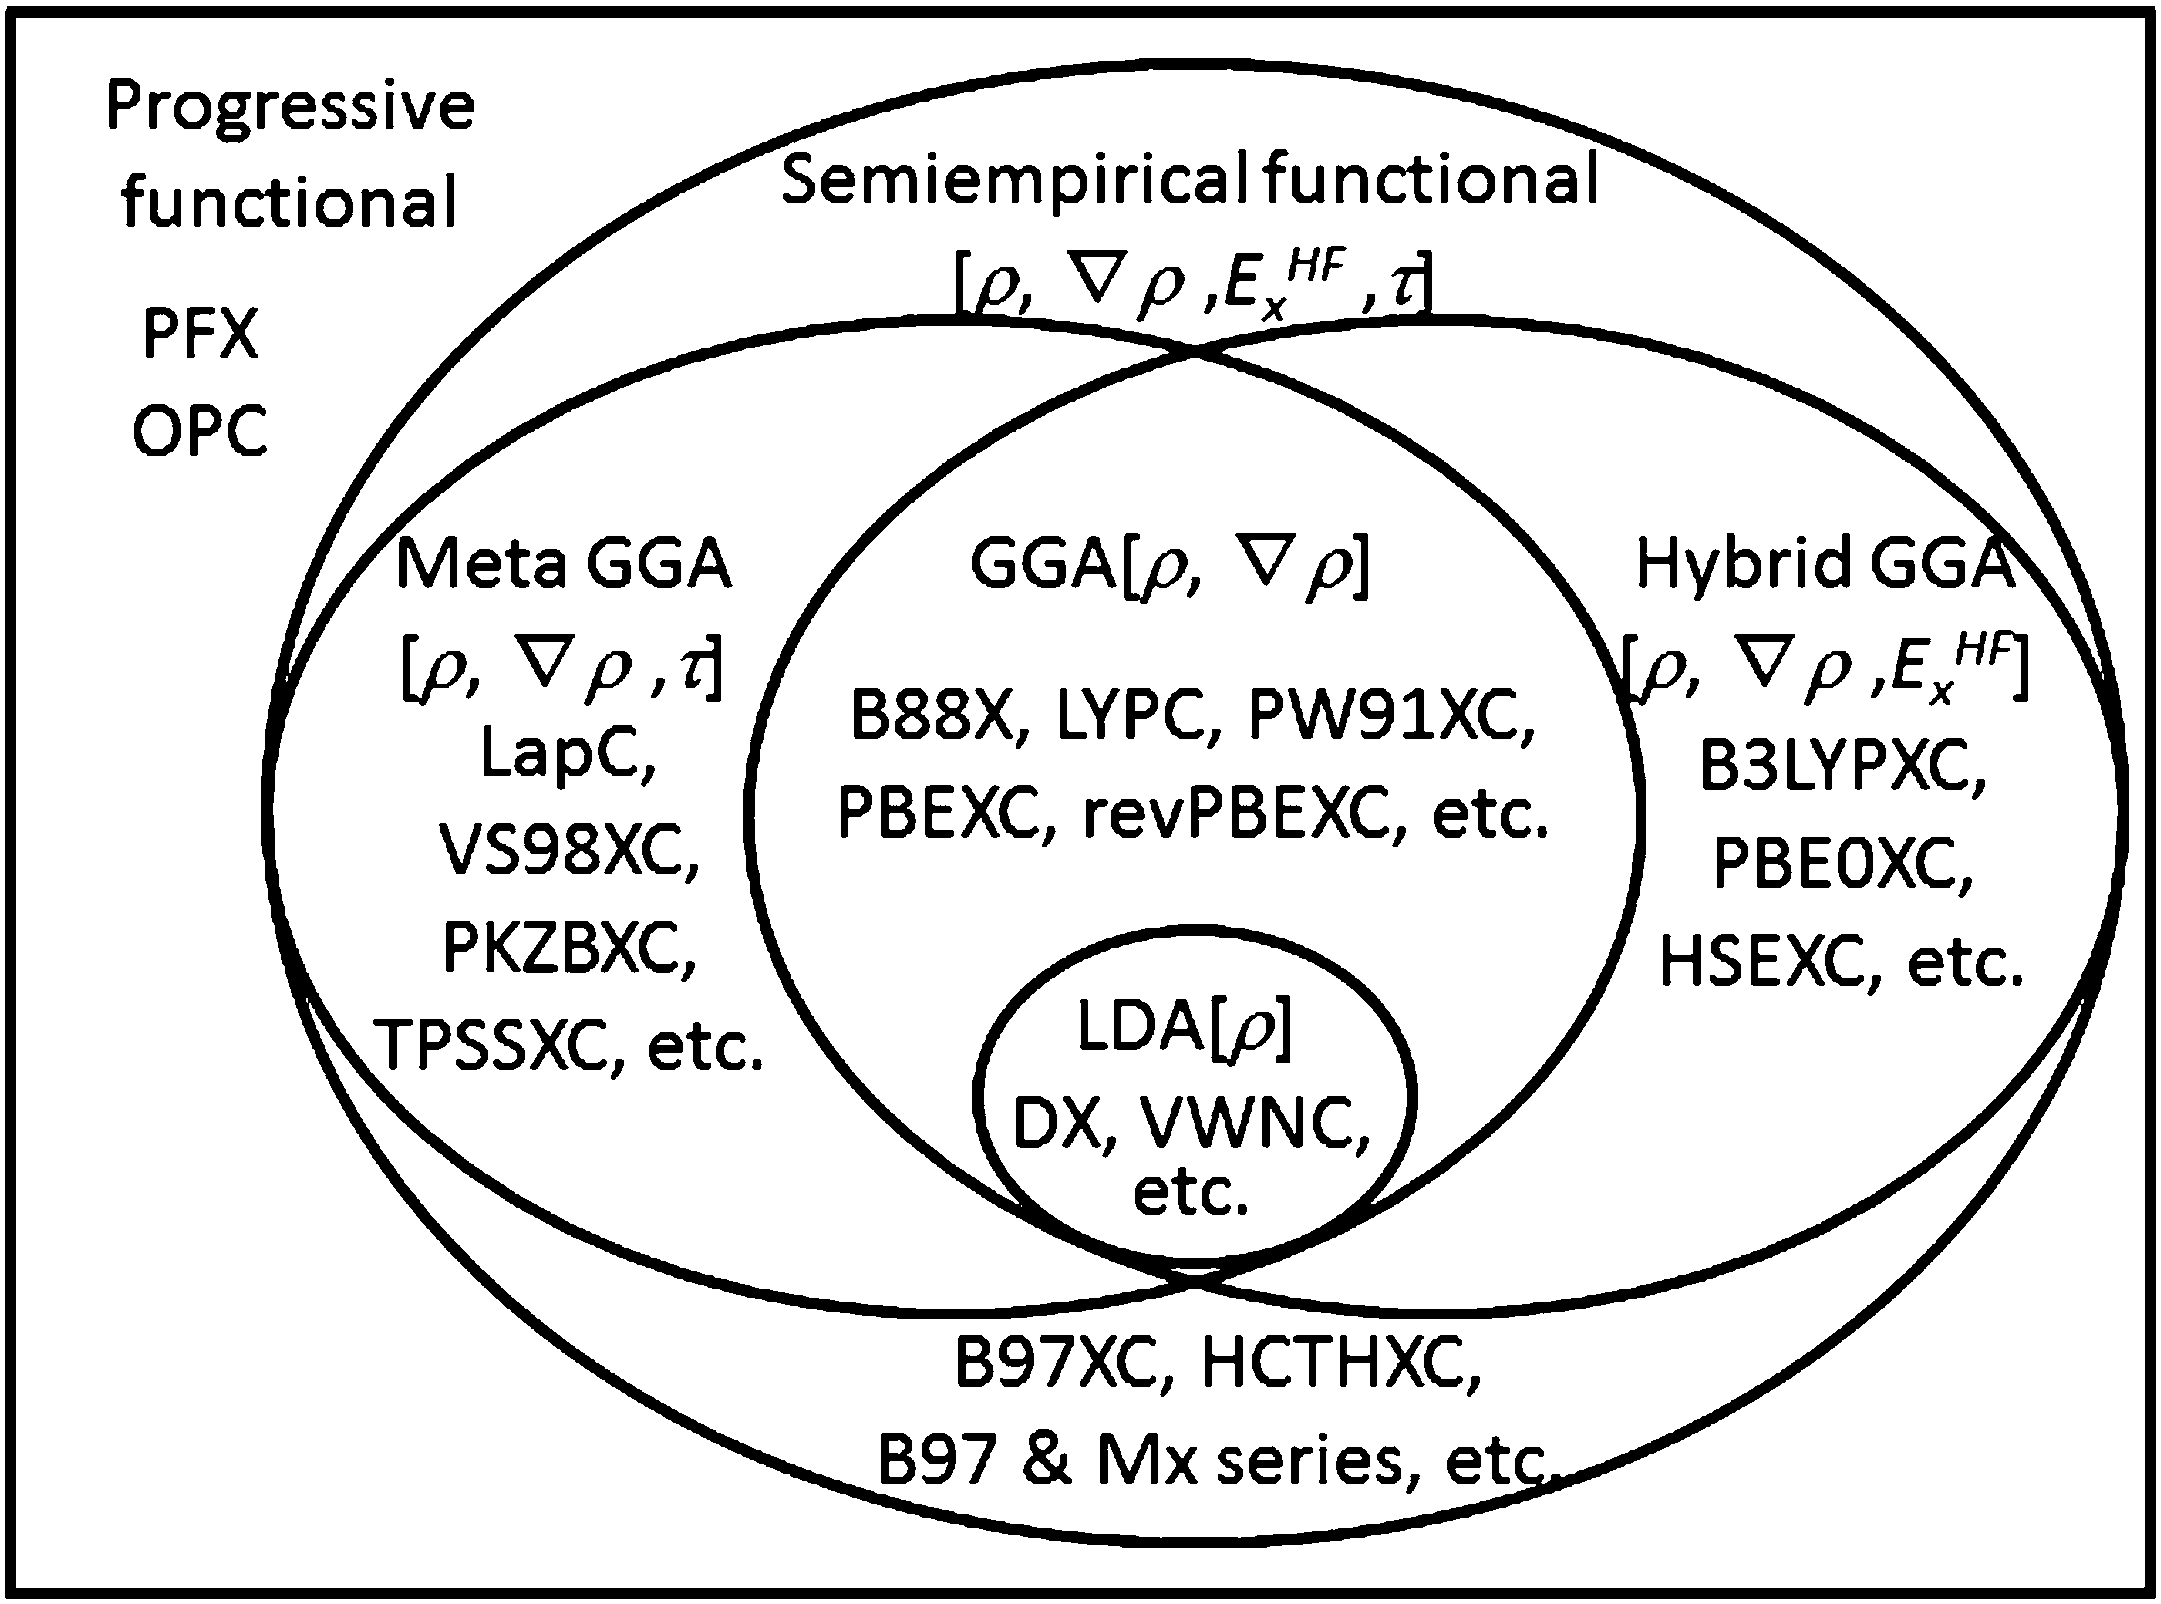
\includegraphics[width=0.5\textwidth]{functional-classification.png}
    \caption{交换-关联泛函的分类}
    \label{fig:excahnge-correlation-functional}
\end{figure}

\subsection{LDA近似}

当电子密度变化非常平缓时,$\grad{\rho},\laplacian{\rho}$等全部可以看成是零,此时交换关联泛函的形式是
\begin{equation}
    E_\text{XC}[\rho(\vb*{r})] = \int \dd[3]{\vb*{r}} \rho(\vb*{r}) \epsilon_\text{XC}(\rho(\vb*{r})).
\end{equation}
这就是所谓的局域密度近似:每单位的交换关联能只和该地点的电子密度有关。

首先我们尝试找一个适用于均匀自由电子气的交换关联泛函。我们取它为均匀自由电子气的基态的交换能加关联能就可以,即
\begin{equation}
    E_\text{XC}[\rho] = E_\text{X}[\rho] + E_\text{C}[\rho].
\end{equation}
自由电子气的基态就是费米面以内的每个轨道都占据了一上一下两个电子的状态,我们设共有$N$个电子,那么这些电子占据了$N/2$个不同的轨道。设这些轨道为$\{\phi_i(\vb*{r})\}$。
仅考虑库伦相互作用引入的一阶微扰,则有
\[
    E = \sum_{\sigma, \sigma'} \mel{\Psi}{
        \frac{1}{2} \int \dd[3]{\vb*{r}} \dd[3]{\vb*{r}'} {\psi}^\dagger_{\sigma}(\vb*{r}) {\psi}^\dagger_{\sigma'}(\vb*{r}') \frac{1}{\abs{\vb*{r} - \vb*{r}'}} {\psi}_{\sigma'}(\vb*{r}') {\psi}_\sigma(\vb*{r})
    }{\Psi}.
\]
这里必须完整地考虑自旋自由度的作用。可以使用Wick定理把上式展开,从而得到Hartree-Fock近似型的表达式。
请注意由于均匀电子气中没有自旋翻转,任何形如
\[
    \mel{\Psi}{{\psi}_\sigma^\dagger {\psi}_{\sigma'}}{\Psi}, \quad \sigma \neq \sigma'
\]
的项都是零,而
\[
    \mel{\Psi}{{\psi}^\dagger_\sigma(\vb*{r}) {\psi}_{\sigma}(\vb*{r}')}{\Psi} = \sum_i \phi_i^*(\vb*{r}) \phi_i(\vb*{r}'),
\]
于是最后能量修正为
\[
    E = \frac{1}{2} \int \dd[3]{\vb*{r}} \dd[3]{\vb*{r}'} \frac{1}{\abs{\vb*{r} - \vb*{r}'}} \bigg(
        \underbrace{4 \sum_{i} \abs{\phi_i(\vb*{r})}^2 \sum_{i} \abs{\phi_i(\vb*{r}')}^2}_\text{classical coulomb energy} - \underbrace{2 \sum_i \phi_i^*(\vb*{r}) \phi_i(\vb*{r}') \sum_i \phi_i^*(\vb*{r}') \phi_i(\vb*{r})}_\text{exchange energy}
    \bigg).
\]
交换能项前面的因子是$2$而不是$4$是因为自旋不同的电子之间的交换能全部抵消了。这样交换能就是
\begin{equation}
    E_\text{X} = - \int \dd[3]{\vb*{r}} \dd[3]{\vb*{r}'} \frac{1}{\abs{\vb*{r} - \vb*{r}'}} \abs{\sum_i \phi_i^*(\vb*{r}) \phi_i(\vb*{r}')}^2 . 
    \label{eq:exchange-energy-homogeneous-gas}
\end{equation}
对箱归一化的均匀电子气,有
\[
    \phi_i(\vb*{r}) = \frac{1}{\sqrt{V}} \ee^{- \ii \vb*{k}_i \cdot \vb*{r}},
\]
于是就有
\begin{equation}
    \sum_i \phi_i^*(\vb*{r}) \phi_i(\vb*{r}') = \sum_{\text{occupied $\vb*{k}$}} \frac{1}{V} \ee^{\ii \vb*{k} \cdot (\vb*{r} - \vb*{r}')} = \frac{1}{(2\pi)^3} \int_{\abs{\vb*{k}} < k_\text{F}} \dd[3]{\vb*{k}} \ee^{\ii \vb*{k} \cdot (\vb*{r} - \vb*{r}')},
    \label{eq:homogeneous-density}
\end{equation}
特别的,电子密度的一半(因为只考虑了轨道自由度)为
\[
    n(\vb*{r}) / 2 = \frac{k_\text{F}^3}{6 \pi^2}.
\]
上式代入\eqref{eq:exchange-energy-homogeneous-gas}就得到交换能的形式。
在这里我们稍微做一些推广。考虑一个非均匀的自由电子气,其非均匀性可能来自一些杂质或者特殊的相互作用,总之,每一个宏观小微观大的体积元可以看成一个用于归一化波函数的箱子,波函数定域在这个箱子里面(杂质会导致局域化)。
这样只有$\vb*{r} - \vb*{r}'$不超出一个箱子时\eqref{eq:homogeneous-density}才有明显的非零值。
每个箱子都有自己的费米动量,记作$k_\text{F}(\vb*{r})$(具体是关于$\vb*{r}$还是$\vb*{r}'$无关紧要因为两者总是在同一个箱子内)。
令
\[
    \vb*{s} = \vb*{r} - \vb*{r}', 
\]
则
\[
    \begin{aligned}
        E_\text{X} &= - \int \dd[3]{\vb*{r}} \dd[3]{\vb*{s}} \frac{1}{s} \left( \frac{1}{(2\pi)^3} \int_{\abs{\vb*{k}} < k_\text{F}} \dd[3]{\vb*{k}} \ee^{\ii \vb*{k} \cdot \vb*{s}} \right)^2 \\
        &= - \int \dd[3]{\vb*{r}} \dd[3]{\vb*{s}} \frac{1}{s} \left( \frac{3}{2} \frac{\sin t - t \cos t}{t^3} n(\vb*{r}) \right)^2 \quad (t= k_\text{F}(\vb*{r}) s) \\
        &= - 9 \pi \int \dd[3]{\vb*{r}} \int \dd{t} \frac{t}{k_\text{F}(\vb*{r})^2} n(\vb*{r})^2 \left( \frac{\sin t - t \cos t}{t^3} \right)^2 \\
        &= - \frac{3}{4} \left( \frac{3}{\pi} \right)^{1/3} \int \dd[3]{\vb*{r}} \rho(\vb*{r})^{4/3}.
    \end{aligned}
\]
这就得到了\concept{托马斯-费米-狄拉克泛函}:
\begin{equation}
    E_\text{X}[\rho] = - \frac{3}{4} \left( \frac{3}{\pi} \right)^{1/3} \int \dd[3]{\vb*{r}} \rho(\vb*{r})^{4/3} = - 0.7386 \int \dd[3]{\vb*{r}} \rho(\vb*{r})^{4/3}
\end{equation}
对均匀或不均匀但缓变的电子气这个泛函适用。

\subsection{GGA近似}

\section{计算步骤}

\autoref{alg:basic-kohn-sham}给出的只是求解\eqref{eq:kohn-sham-eq}的方法,而实际的凝聚态计算还需要考虑原子核的位置、携带的电荷(从而确定材料中的电子总量)等信息。
本节给出几种常见的DFT计算任务。

\subsection{基于超胞的平面波DFT计算}\label{sec:supercell-pwdft}

\eqref{eq:kohn-sham-eq}中涉及的单电子波函数的个数要和系统中电子的数目一样多,否则$\rho(\vb*{r})$的总量不正确。
介质中的电子数目是非常多的,从而直接求解\eqref{eq:kohn-sham-eq}并不现实。
晶体有周期性结构,这就大大简化了计算。实际上,由于相互作用衰减得很快,我们完全可以假定液体等也有周期性边界条件,只不过此时的晶胞要取得非常大。

于是以下我们将DFT计算中被认为是周期性的单元称为\concept{超胞(supercell)},对固体通常要求超胞取最简单的形式,即原胞,对单分子、液体或是有杂质的系统等则需要取一个较大的超胞。
对杂质,超胞应该包括杂质周围足够大的体态。
对单分子,当超胞足够大时第一布里渊区足够小,从而计算出的所谓“能带”实际上和单独的一个个能级毫无区别。
我们需要指定超胞的几何形状,并且在超胞内给出各个原子核的位置。

由于\eqref{eq:kohn-sham-eq}此时就是周期性的,它的解——也就是$\phi_i(\vb*{r})$——可以看成某个以我们设定的超胞为原胞的晶体中的单电子波函数,从而Bloch定理\eqref{eq:bloch-wavefunction}成立,且$\phi_i(\vb*{r})$中的$i$应该替换成Bloch波矢$\vb*{k}$和能带标记$n$。
由于\eqref{eq:bloch-wavefunction}中的$u(\vb*{r})$具有周期性,它可以被展开成用倒格矢标记的一系列傅里叶分量,因此我们有
\begin{equation}
    \phi_{n \vb*{k}}(\vb*{r}) = \sum_{\vb*{G}} c_{n, \vb*{k}, \vb*{G}} \ee^{\ii (\vb*{k} + \vb*{G}) \cdot \vb*{r}},
\end{equation}
或者,考虑到$\vb*{k}$局限在第一布里渊区中而$\vb*{G}$是倒格矢,从$\vb*{k} + \vb*{G}$可以唯一确定$\vb*{k}$和$\vb*{G}$,有
\begin{equation}
    \phi_{n \vb*{k}}(\vb*{r}) = \sum_{\vb*{G}} c_{n, \vb*{k} + \vb*{G}} \ee^{\ii (\vb*{k} + \vb*{G}) \cdot \vb*{r}}.
\end{equation}
这种选取$\phi_i$的方法称为\concept{平面波DFT(PWDFT)}。

上式的$\vb*{G}$分量在\eqref{eq:kohn-sham-eq}的动能项部分为$(\vb*{k} + \vb*{G})^2 / 2m$,由于实际能够存储的傅里叶分量的个数是有限的,通常会引入一个\concept{截断能},对每个$\vb*{k}$,我们只保留对动能的贡献小于截断能的那些$\vb*{G}$。
这意味着我们忽略了空间尺度特别小的现象,并且忽略了一部分能量,但是如果对应的$c_{n, \vb*{k} + \vb*{G}}$不大就没有什么问题。

实际能够处理的晶体都是有限大小的,或者说实际的$\vb*{k}$的取值是第一布里渊区中离散的一些点。
这就是说,我们需要给出一种“第一布里渊区中的动量采样”。
显然,采样越密越好;可以使用$\vb*{k} \cdot \vb*{p}$来简化计算。

最后我们处理至今尚未提及的$V_\text{ext}$。如\autoref{sec:pseudopotential}所述,外层电子感受到的势场可以用赝势取代。
这里我们有好几种可能的做法:可以只计算外层电子,完全不计算内层电子,从而自始至终$V_\text{ext}$都是用赝势组合而成的。此时截断能可以设置得比较小,因为$\phi_{n \vb*{k}}(\vb*{r})$在靠近原子核的位置也不会发生剧烈振荡。
也可以用赝势计算出初步的电子密度,然后改用库伦势做进一步计算。

\begin{algorithm}

    \DontPrintSemicolon
    \SetAlgoLined

    \KwData{初始电子密度$\rho_0(\vb*{r})$,交换关联泛函选取$E_\text{XC}[\rho(\vb*{r})]$,不同原子的赝势,$\vb*{k}$点采样$K = \{\vb*{k}\}$,截断能$E_\text{cut}$,最大迭代次数$N_\text{max}$,容差$\epsilon$}
    \KwResult{Kohn-Sham波函数$\phi_{n \vb*{k}}(\vb*{r})$和对应的本征值$\epsilon_{n \vb*{k}}$}
    
    \For{$\vb*{k} \in K$}{
        根据$\frac{(\vb*{k} + \vb*{G})^2}{2m} < E_\text{cut}$确定 \;
    } % TODO:

    $i = 1$ \;
    使用不同原子的赝势构造\eqref{eq:kohn-sham-eq}中的$V_\text{ext}$ \;
    将$\rho_0(\vb*{r})$代入\eqref{eq:kohn-sham-eq}求解得到$\phi_n^{(1)}$和$\epsilon_n^{(1)}$ \;
    将$\phi_n^{(1)}$代入\eqref{eq:kohn-sham-density}计算得到$\rho_1(\vb*{r})$ \;
    \While{$\rho_i(\vb*{r})$和$\rho_{i-1}(\vb*{r})$的差别大于容差$\epsilon$且$i < N_\text{max}$}{
        将$\rho_i$代入\eqref{eq:kohn-sham-eq}求解得到$\phi_n^{(i+1)}$和$\epsilon_n^{(i+1)}$ \;
        $i = i + 1$ \;
    }
    
    \Return{波函数$\phi^{(i)}_n$和本征值$\epsilon^{(i)}_n$}\;

    \caption{给定晶格和原子赝势的PWDFT计算}
    \label{alg:static-pwdft}
\end{algorithm}

将以上考虑放进\autoref{alg:basic-kohn-sham}中,我们得到\autoref{alg:static-pwdft},即所谓\concept{静态自洽计算}。
只要输入的晶体结构是准确的,交换关联泛函的质量足够好,我们就得到了外层电子或是全电子(一般来说用不到,因为化学反应的能级不足以激发内层电子,倒是从头计算赝势时需要全电子计算)的模拟结果:这其中没有引入任何经验参数,并且每一条可能的能带都纳入了考虑。
虽然如此,截断能、$\vb*{k}$点采样、赝势的选择仍然会显著影响计算精度。

有时候我们对晶体结构只有一个大概的猜测,此时需要做结构优化,即所谓\concept{结构优化自洽计算}。
